\section{System Requirements}
The following table lists the user requirements from the original system request.
\begin{enumerate}
	\item The system shall allow the unique user identification
	\item The system shall ask for username and password to access it
	\item The system shall identify a special user as administrator who will be able to
	\begin{enumerate}
		\item Add other users to the system.
		\item Permanently delete objects from the system.
		\item recover user deleted items.
		\item block users from loggin in.
		\item Unblock the users blocked.
	\end{enumerate}
	\item The system shall allow to list, create, modify and delete ''projects'' to group link checker items.
	\item The system shall allow to list, create, modify and delete ''link checker'' items.
	\item The system shall check the link status automatically when displaying the checker list
	\item The system must be developed in PHP
	\item The system could be developed using the Laravel framework.
	\item The system will have an admin template in use for it's display.
\end{enumerate}

\section{System Design}

\subsection{Entity Relationship Diagram}

\subsection{Use Cases}

\begin{figure}[ht!]
	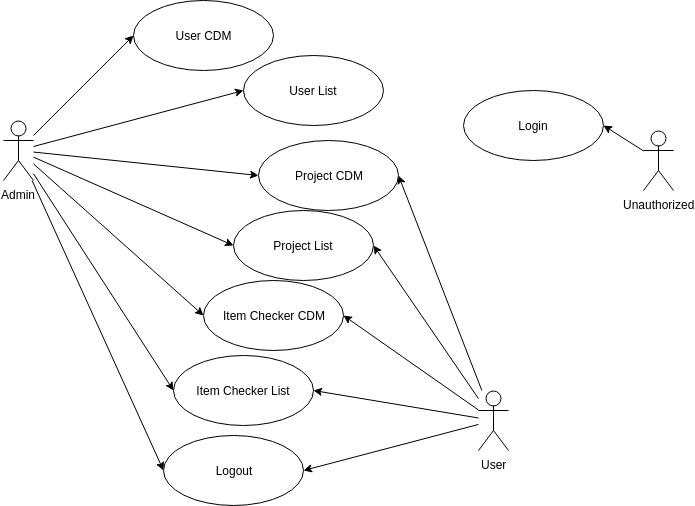
\includegraphics[width=\textwidth]{images/Use-Cases-Linkchecker}
	\caption{System use cases}
\end{figure}

\subsection{Design desitions}
\begin{itemize}
	\item The link checker items list will be paged
	\item The link checker items page will have 15 items by default, 25 as a second option and 50 as the last one.
	\item The Angular library will be used for the interface wherever it applies.
\end{itemize}